
\INEchaptercarta{Caracterización escolar de la población económicamente activa}{}


\cajita{Participación PEA}{La tasa de participación de la población económicamente activa, es el porcentaje de las personas que están ocupadas o en desempleo abierto en relación al total de la población que está en edad para trabajar (mayor a 14 años), llamada también PET. 
		
	En el 2014, el 60.5\% de la PET estaba trabajando o en desempleo abierto.}{Tasa de participación de la población económicamente activa}{República de Guatemala, serie histórica, en porcentaje}{\ \\[0mm]\begin{tikzpicture}[x=1pt,y=1pt]  % Created by tikzDevice version 0.9 on 2015-12-11 10:47:35
% !TEX encoding = UTF-8 Unicode
\definecolor{fillColor}{RGB}{255,255,255}
\path[use as bounding box,fill=fillColor,fill opacity=0.00] (0,0) rectangle (289.08,198.74);
\begin{scope}
\path[clip] (  0.00,  0.00) rectangle (289.08,198.74);

\path[] (  0.00,  0.00) rectangle (289.08,198.74);
\end{scope}
\begin{scope}
\path[clip] (  0.00,  0.00) rectangle (289.08,198.74);

\path[] (  1.64, 17.78) rectangle (280.54,191.48);

\path[] (  1.64, 49.89) --
	(280.54, 49.89);

\path[] (  1.64, 98.34) --
	(280.54, 98.34);

\path[] (  1.64,146.79) --
	(280.54,146.79);

\path[] (  1.64, 25.67) --
	(280.54, 25.67);

\path[] (  1.64, 74.12) --
	(280.54, 74.12);

\path[] (  1.64,122.56) --
	(280.54,122.56);

\path[] (  1.64,171.01) --
	(280.54,171.01);

\path[] ( 41.49, 17.78) --
	( 41.49,191.48);

\path[] (107.89, 17.78) --
	(107.89,191.48);

\path[] (174.30, 17.78) --
	(174.30,191.48);

\path[] (240.70, 17.78) --
	(240.70,191.48);
\definecolor{drawColor}{RGB}{0,0,255}

\path[draw=drawColor,line width= 1.7pt,line join=round] ( 41.49,174.40) --
	(107.89,183.59) --
	(174.30,171.35) --
	(240.70,171.25);
\definecolor{drawColor}{RGB}{0,0,0}

\node[text=drawColor,anchor=base,inner sep=0pt, outer sep=0pt, scale=  1.01] at ( 41.49,162.53) {61.4};

\node[text=drawColor,anchor=base,inner sep=0pt, outer sep=0pt, scale=  1.01] at (107.89,187.54) {65.2};

\node[text=drawColor,anchor=base west,inner sep=0pt, outer sep=0pt, scale=  1.01] at (174.30,175.31) {60.1};

\node[text=drawColor,anchor=base,inner sep=0pt, outer sep=0pt, scale=  1.01] at (240.70,159.38) {60.1};

\path[draw=drawColor,line width= 0.1pt,line join=round] (  1.64, 25.67) -- (280.54, 25.67);

\path[] (  1.64, 17.78) rectangle (280.54,191.48);
\end{scope}
\begin{scope}
\path[clip] (  0.00,  0.00) rectangle (289.08,198.74);

\path[] (  1.64, 17.78) --
	(  1.64,191.48);
\end{scope}
\begin{scope}
\path[clip] (  0.00,  0.00) rectangle (289.08,198.74);

\path[] (  0.00, 25.67) --
	(  1.64, 25.67);

\path[] (  0.00, 74.12) --
	(  1.64, 74.12);

\path[] (  0.00,122.56) --
	(  1.64,122.56);

\path[] (  0.00,171.01) --
	(  1.64,171.01);
\end{scope}
\begin{scope}
\path[clip] (  0.00,  0.00) rectangle (289.08,198.74);

\path[] (  1.64, 17.78) --
	(280.54, 17.78);
\end{scope}
\begin{scope}
\path[clip] (  0.00,  0.00) rectangle (289.08,198.74);

\path[] ( 41.49, 13.51) --
	( 41.49, 17.78);

\path[] (107.89, 13.51) --
	(107.89, 17.78);

\path[] (174.30, 13.51) --
	(174.30, 17.78);

\path[] (240.70, 13.51) --
	(240.70, 17.78);
\end{scope}
\begin{scope}
\path[clip] (  0.00,  0.00) rectangle (289.08,198.74);
\definecolor{drawColor}{RGB}{0,0,0}

\node[text=drawColor,anchor=base,inner sep=0pt, outer sep=0pt, scale=  1.00] at ( 41.49,  2.85) {2011};

\node[text=drawColor,anchor=base,inner sep=0pt, outer sep=0pt, scale=  1.00] at (107.89,  2.85) {2012};

\node[text=drawColor,anchor=base,inner sep=0pt, outer sep=0pt, scale=  1.00] at (174.30,  2.85) {2013};

\node[text=drawColor,anchor=base,inner sep=0pt, outer sep=0pt, scale=  1.00] at (240.70,  2.85) {2014};
\end{scope}
  \end{tikzpicture}}{Instituto Nacional de Estadística, con datos de ENEI II-2014}

\cajita{PEA que sabe leer y escribir}{De la población económicamente activa (PEA), en el 2014, el 79.9\% reportó que sabía leer y escribir. La desagregación por dominio de estudio muestra que el 72.9\% la PEA del área rural nacional sabía leer y escribir, siendo el dominio con el menor porcentaje.
	
	Por otro lado, la PEA del área urbana metropolitana con esta habilidad tuvo el 93.2\%.}{Proporción de la población económicamente activa – PEA -, que sabe leer y escribir por dominios de estudio }{República de Guatemala, año 2014, en porcentaje}{\ \\[0mm]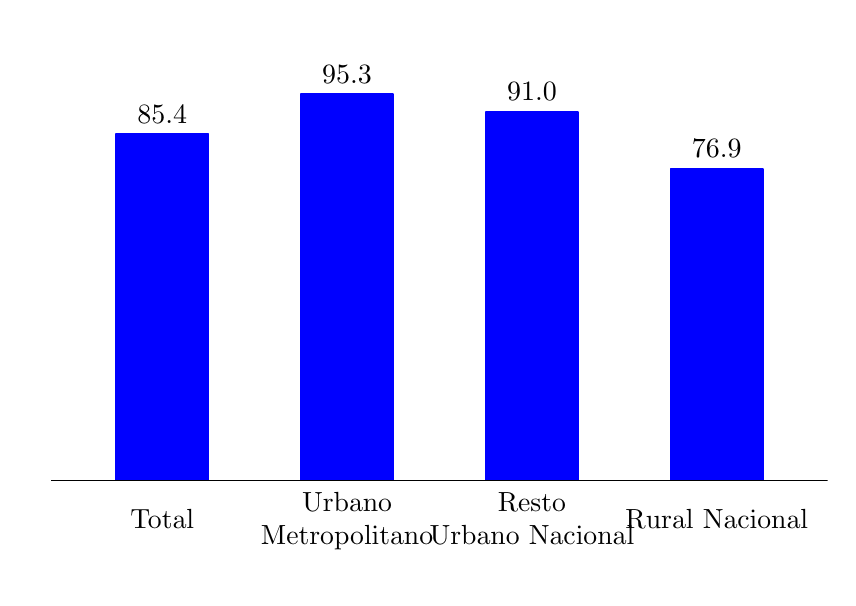
\begin{tikzpicture}[x=1pt,y=1pt]  % Created by tikzDevice version 0.9 on 2015-12-11 10:47:36
% !TEX encoding = UTF-8 Unicode
\definecolor{fillColor}{RGB}{255,255,255}
\path[use as bounding box,fill=fillColor,fill opacity=0.00] (0,0) rectangle (289.08,198.74);
\begin{scope}
\path[clip] (  0.00,  0.00) rectangle (289.08,198.74);

\path[] (  0.00,  0.00) rectangle (289.08,198.74);
\end{scope}
\begin{scope}
\path[clip] (  0.00,  0.00) rectangle (289.08,198.74);

\path[] (  8.54, 28.23) rectangle (289.08,181.67);

\path[] ( 48.61, 28.23) --
	( 48.61,181.67);

\path[] (115.41, 28.23) --
	(115.41,181.67);

\path[] (182.21, 28.23) --
	(182.21,181.67);

\path[] (249.00, 28.23) --
	(249.00,181.67);
\definecolor{drawColor}{RGB}{0,0,255}
\definecolor{fillColor}{RGB}{0,0,255}

\path[draw=drawColor,line width= 0.6pt,line join=round,fill=fillColor] ( 31.91, 35.21) rectangle ( 65.31,160.24);

\path[draw=drawColor,line width= 0.6pt,line join=round,fill=fillColor] ( 98.71, 35.21) rectangle (132.11,174.70);

\path[draw=drawColor,line width= 0.6pt,line join=round,fill=fillColor] (165.51, 35.21) rectangle (198.91,168.34);

\path[draw=drawColor,line width= 0.6pt,line join=round,fill=fillColor] (232.30, 35.21) rectangle (265.70,147.71);
\definecolor{drawColor}{RGB}{0,0,0}

\path[draw=drawColor,line width= 0.1pt,line join=round] (  8.54, 35.21) -- (289.08, 35.21);

\node[text=drawColor,anchor=base,inner sep=0pt, outer sep=0pt, scale=  1.01] at ( 48.61,164.19) {85.4};

\node[text=drawColor,anchor=base,inner sep=0pt, outer sep=0pt, scale=  1.01] at (115.41,178.65) {95.3};

\node[text=drawColor,anchor=base,inner sep=0pt, outer sep=0pt, scale=  1.01] at (182.21,172.29) {91.0};

\node[text=drawColor,anchor=base,inner sep=0pt, outer sep=0pt, scale=  1.01] at (249.00,151.66) {76.9};

\path[] (  8.54, 28.23) rectangle (289.08,181.67);
\end{scope}
\begin{scope}
\path[clip] (  0.00,  0.00) rectangle (289.08,198.74);

\path[] (  8.54, 28.23) --
	(  8.54,181.67);
\end{scope}
\begin{scope}
\path[clip] (  0.00,  0.00) rectangle (289.08,198.74);

\path[] (  8.54, 28.23) --
	(289.08, 28.23);
\end{scope}
\begin{scope}
\path[clip] (  0.00,  0.00) rectangle (289.08,198.74);

\path[] ( 48.61, 23.96) --
	( 48.61, 28.23);

\path[] (115.41, 23.96) --
	(115.41, 28.23);

\path[] (182.21, 23.96) --
	(182.21, 28.23);

\path[] (249.00, 23.96) --
	(249.00, 28.23);
\end{scope}
\begin{scope}
\path[clip] (  0.00,  0.00) rectangle (289.08,198.74);
\definecolor{drawColor}{RGB}{0,0,0}

\node[text=drawColor,anchor=base,inner sep=0pt, outer sep=0pt, scale=  1.00] at ( 48.61, 17.92) {Total};

\node[text=drawColor,anchor=base,inner sep=0pt, outer sep=0pt, scale=  1.00] at (115.41, 23.86) {Urbano };

\node[text=drawColor,anchor=base,inner sep=0pt, outer sep=0pt, scale=  1.00] at (115.41, 11.98) { Metropolitano};

\node[text=drawColor,anchor=base,inner sep=0pt, outer sep=0pt, scale=  1.00] at (182.21, 23.86) {Resto };

\node[text=drawColor,anchor=base,inner sep=0pt, outer sep=0pt, scale=  1.00] at (182.21, 11.98) { Urbano Nacional};

\node[text=drawColor,anchor=base,inner sep=0pt, outer sep=0pt, scale=  1.00] at (249.00, 17.92) {Rural Nacional};
\end{scope}
  \end{tikzpicture}}{Instituto Nacional de Estadística, con datos de ENEI II-2014}

\cajita{PEA según nivel de escolaridad}{La distribución según el último nivel escolar aprobado por la población que es económicamente activa, muestra que el 40.7\% alcanzó hasta el nivel primario. Estudios superiores y de postgrado la tiene el 7.8\% de la PEA.
	
	 Otro indicador importante es que 19.4\% de la población económicamente activa, no ha obtenido ningún grado de escolaridad. }{Distribución de la población económicamente activa, según nivel de escolaridad}{República de Guatemala, año 2014, en porcentaje}{\ \\[0mm]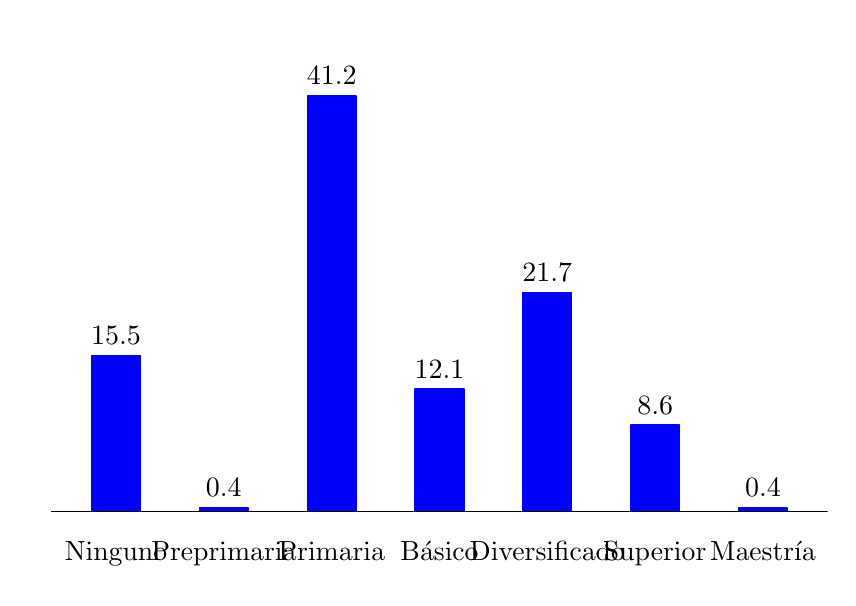
\begin{tikzpicture}[x=1pt,y=1pt]  % Created by tikzDevice version 0.9 on 2015-12-11 10:47:38
% !TEX encoding = UTF-8 Unicode
\definecolor{fillColor}{RGB}{255,255,255}
\path[use as bounding box,fill=fillColor,fill opacity=0.00] (0,0) rectangle (289.08,198.74);
\begin{scope}
\path[clip] (  0.00,  0.00) rectangle (289.08,198.74);

\path[] (  0.00,  0.00) rectangle (289.08,198.74);
\end{scope}
\begin{scope}
\path[clip] (  0.00,  0.00) rectangle (289.08,198.74);

\path[] (  8.54, 16.35) rectangle (289.08,181.67);

\path[] ( 31.91, 16.35) --
	( 31.91,181.67);

\path[] ( 70.88, 16.35) --
	( 70.88,181.67);

\path[] (109.84, 16.35) --
	(109.84,181.67);

\path[] (148.81, 16.35) --
	(148.81,181.67);

\path[] (187.77, 16.35) --
	(187.77,181.67);

\path[] (226.74, 16.35) --
	(226.74,181.67);

\path[] (265.70, 16.35) --
	(265.70,181.67);
\definecolor{drawColor}{RGB}{0,0,255}
\definecolor{fillColor}{RGB}{0,0,255}

\path[draw=drawColor,line width= 0.6pt,line join=round,fill=fillColor] ( 23.15, 23.87) rectangle ( 40.68, 80.27);

\path[draw=drawColor,line width= 0.6pt,line join=round,fill=fillColor] ( 62.11, 23.87) rectangle ( 79.65, 25.20);

\path[draw=drawColor,line width= 0.6pt,line join=round,fill=fillColor] (101.08, 23.87) rectangle (118.61,174.16);

\path[draw=drawColor,line width= 0.6pt,line join=round,fill=fillColor] (140.04, 23.87) rectangle (157.57, 68.07);

\path[draw=drawColor,line width= 0.6pt,line join=round,fill=fillColor] (179.01, 23.87) rectangle (196.54,103.04);

\path[draw=drawColor,line width= 0.6pt,line join=round,fill=fillColor] (217.97, 23.87) rectangle (235.50, 55.10);

\path[draw=drawColor,line width= 0.6pt,line join=round,fill=fillColor] (256.93, 23.87) rectangle (274.47, 25.27);
\definecolor{drawColor}{RGB}{0,0,0}

\path[draw=drawColor,line width= 0.1pt,line join=round] (  8.54, 23.87) -- (289.08, 23.87);

\node[text=drawColor,anchor=base,inner sep=0pt, outer sep=0pt, scale=  1.01] at ( 31.91, 84.23) {15.5};

\node[text=drawColor,anchor=base,inner sep=0pt, outer sep=0pt, scale=  1.01] at ( 70.88, 29.16) {0.4};

\node[text=drawColor,anchor=base,inner sep=0pt, outer sep=0pt, scale=  1.01] at (109.84,178.11) {41.2};

\node[text=drawColor,anchor=base,inner sep=0pt, outer sep=0pt, scale=  1.01] at (148.81, 72.03) {12.1};

\node[text=drawColor,anchor=base,inner sep=0pt, outer sep=0pt, scale=  1.01] at (187.77,107.00) {21.7};

\node[text=drawColor,anchor=base,inner sep=0pt, outer sep=0pt, scale=  1.01] at (226.74, 59.06) {8.6};

\node[text=drawColor,anchor=base,inner sep=0pt, outer sep=0pt, scale=  1.01] at (265.70, 29.23) {0.4};

\path[] (  8.54, 16.35) rectangle (289.08,181.67);
\end{scope}
\begin{scope}
\path[clip] (  0.00,  0.00) rectangle (289.08,198.74);

\path[] (  8.54, 16.35) --
	(  8.54,181.67);
\end{scope}
\begin{scope}
\path[clip] (  0.00,  0.00) rectangle (289.08,198.74);

\path[] (  8.54, 16.35) --
	(289.08, 16.35);
\end{scope}
\begin{scope}
\path[clip] (  0.00,  0.00) rectangle (289.08,198.74);

\path[] ( 31.91, 12.08) --
	( 31.91, 16.35);

\path[] ( 70.88, 12.08) --
	( 70.88, 16.35);

\path[] (109.84, 12.08) --
	(109.84, 16.35);

\path[] (148.81, 12.08) --
	(148.81, 16.35);

\path[] (187.77, 12.08) --
	(187.77, 16.35);

\path[] (226.74, 12.08) --
	(226.74, 16.35);

\path[] (265.70, 12.08) --
	(265.70, 16.35);
\end{scope}
\begin{scope}
\path[clip] (  0.00,  0.00) rectangle (289.08,198.74);
\definecolor{drawColor}{RGB}{0,0,0}

\node[text=drawColor,anchor=base,inner sep=0pt, outer sep=0pt, scale=  1.00] at ( 31.91,  6.04) {Ninguno};

\node[text=drawColor,anchor=base,inner sep=0pt, outer sep=0pt, scale=  1.00] at ( 70.88,  6.04) {Preprimaria};

\node[text=drawColor,anchor=base,inner sep=0pt, outer sep=0pt, scale=  1.00] at (109.84,  6.04) {Primaria};

\node[text=drawColor,anchor=base,inner sep=0pt, outer sep=0pt, scale=  1.00] at (148.81,  6.04) {Básico};

\node[text=drawColor,anchor=base,inner sep=0pt, outer sep=0pt, scale=  1.00] at (187.77,  6.04) {Diversificado};

\node[text=drawColor,anchor=base,inner sep=0pt, outer sep=0pt, scale=  1.00] at (226.74,  6.04) {Superior};

\node[text=drawColor,anchor=base,inner sep=0pt, outer sep=0pt, scale=  1.00] at (265.70,  6.04) {Maestría};
\end{scope}
  \end{tikzpicture} }{Instituto Nacional de Estadística, con datos de ENEI II-2014}



\cajita{PEA según escolaridad y sexo}{Las distribuciones de la población económicamente activa por hombre y mujer, muestra que ambos grupos tiene un mayor porcentaje con educación primaria.
	
	El 10.9\% de las mujeres que forman parte de la PEA tienen estudios superiores o de postgrado.}{Distribución de la población económicamente activa por sexo según nivel de escolaridad}{República de Guatemala, año 2014, en porcentaje}{\ \\[0mm]\begin{tikzpicture}[x=1pt,y=1pt]  % Created by tikzDevice version 0.9 on 2015-12-11 10:47:39
% !TEX encoding = UTF-8 Unicode
\definecolor{fillColor}{RGB}{255,255,255}
\path[use as bounding box,fill=fillColor,fill opacity=0.00] (0,0) rectangle (289.08,198.74);
\begin{scope}
\path[clip] (  0.00,  0.00) rectangle (289.08,198.74);

\path[] (  0.00,  0.00) rectangle (289.08,198.74);
\end{scope}
\begin{scope}
\path[clip] (  0.00,  0.00) rectangle (289.08,198.74);

\path[] (  7.11, 20.62) rectangle (289.08,172.85);

\path[] ( 30.61, 20.62) --
	( 30.61,172.85);

\path[] ( 69.77, 20.62) --
	( 69.77,172.85);

\path[] (108.93, 20.62) --
	(108.93,172.85);

\path[] (148.10, 20.62) --
	(148.10,172.85);

\path[] (187.26, 20.62) --
	(187.26,172.85);

\path[] (226.42, 20.62) --
	(226.42,172.85);

\path[] (265.58, 20.62) --
	(265.58,172.85);
\definecolor{drawColor}{RGB}{0,0,255}
\definecolor{fillColor}{RGB}{0,0,255}

\path[draw=drawColor,line width= 0.6pt,line join=round,fill=fillColor] ( 15.44, 20.62) rectangle ( 28.16, 71.37);
\definecolor{drawColor}{RGB}{157,187,255}
\definecolor{fillColor}{RGB}{157,187,255}

\path[draw=drawColor,line width= 0.6pt,line join=round,fill=fillColor] ( 33.06, 20.62) rectangle ( 45.79, 77.03);
\definecolor{drawColor}{RGB}{0,0,255}
\definecolor{fillColor}{RGB}{0,0,255}

\path[draw=drawColor,line width= 0.6pt,line join=round,fill=fillColor] ( 54.60, 20.62) rectangle ( 67.32, 21.74);
\definecolor{drawColor}{RGB}{157,187,255}
\definecolor{fillColor}{RGB}{157,187,255}

\path[draw=drawColor,line width= 0.6pt,line join=round,fill=fillColor] ( 72.22, 20.62) rectangle ( 84.95, 22.10);
\definecolor{drawColor}{RGB}{0,0,255}
\definecolor{fillColor}{RGB}{0,0,255}

\path[draw=drawColor,line width= 0.6pt,line join=round,fill=fillColor] ( 93.76, 20.62) rectangle (106.49,172.85);
\definecolor{drawColor}{RGB}{157,187,255}
\definecolor{fillColor}{RGB}{157,187,255}

\path[draw=drawColor,line width= 0.6pt,line join=round,fill=fillColor] (111.38, 20.62) rectangle (124.11,139.29);
\definecolor{drawColor}{RGB}{0,0,255}
\definecolor{fillColor}{RGB}{0,0,255}

\path[draw=drawColor,line width= 0.6pt,line join=round,fill=fillColor] (132.92, 20.62) rectangle (145.65, 65.23);
\definecolor{drawColor}{RGB}{157,187,255}
\definecolor{fillColor}{RGB}{157,187,255}

\path[draw=drawColor,line width= 0.6pt,line join=round,fill=fillColor] (150.54, 20.62) rectangle (163.27, 55.84);
\definecolor{drawColor}{RGB}{0,0,255}
\definecolor{fillColor}{RGB}{0,0,255}

\path[draw=drawColor,line width= 0.6pt,line join=round,fill=fillColor] (172.08, 20.62) rectangle (184.81, 86.45);
\definecolor{drawColor}{RGB}{157,187,255}
\definecolor{fillColor}{RGB}{157,187,255}

\path[draw=drawColor,line width= 0.6pt,line join=round,fill=fillColor] (189.71, 20.62) rectangle (202.43,109.86);
\definecolor{drawColor}{RGB}{0,0,255}
\definecolor{fillColor}{RGB}{0,0,255}

\path[draw=drawColor,line width= 0.6pt,line join=round,fill=fillColor] (211.25, 20.62) rectangle (223.97, 45.30);
\definecolor{drawColor}{RGB}{157,187,255}
\definecolor{fillColor}{RGB}{157,187,255}

\path[draw=drawColor,line width= 0.6pt,line join=round,fill=fillColor] (228.87, 20.62) rectangle (241.60, 58.22);
\definecolor{drawColor}{RGB}{0,0,255}
\definecolor{fillColor}{RGB}{0,0,255}

\path[draw=drawColor,line width= 0.6pt,line join=round,fill=fillColor] (250.41, 20.62) rectangle (263.14, 21.93);
\definecolor{drawColor}{RGB}{157,187,255}
\definecolor{fillColor}{RGB}{157,187,255}

\path[draw=drawColor,line width= 0.6pt,line join=round,fill=fillColor] (268.03, 20.62) rectangle (280.76, 21.94);
\definecolor{drawColor}{RGB}{0,0,0}

\path[draw=drawColor,line width= 0.6pt,line join=round] (  7.11, 20.62) -- (289.08, 20.62);

\node[text=drawColor,anchor=base,inner sep=0pt, outer sep=0pt, scale=  0.82] at ( 21.80, 74.59) {14.9};

\node[text=drawColor,anchor=base,inner sep=0pt, outer sep=0pt, scale=  0.82] at ( 39.42, 80.25) {16.5};

\node[text=drawColor,anchor=base,inner sep=0pt, outer sep=0pt, scale=  0.82] at ( 60.96, 24.96) {0.3};

\node[text=drawColor,anchor=base,inner sep=0pt, outer sep=0pt, scale=  0.82] at ( 78.58, 25.32) {0.4};

\node[text=drawColor,anchor=base,inner sep=0pt, outer sep=0pt, scale=  0.82] at (100.12,176.07) {44.6};

\node[text=drawColor,anchor=base,inner sep=0pt, outer sep=0pt, scale=  0.82] at (117.75,142.51) {34.8};

\node[text=drawColor,anchor=base,inner sep=0pt, outer sep=0pt, scale=  0.82] at (139.29, 68.45) {13.1};

\node[text=drawColor,anchor=base,inner sep=0pt, outer sep=0pt, scale=  0.82] at (156.91, 59.06) {10.3};

\node[text=drawColor,anchor=base,inner sep=0pt, outer sep=0pt, scale=  0.82] at (178.45, 89.67) {19.3};

\node[text=drawColor,anchor=base,inner sep=0pt, outer sep=0pt, scale=  0.82] at (196.07,113.08) {26.2};

\node[text=drawColor,anchor=base,inner sep=0pt, outer sep=0pt, scale=  0.82] at (217.61, 48.52) {7.2};

\node[text=drawColor,anchor=base,inner sep=0pt, outer sep=0pt, scale=  0.82] at (235.23, 61.44) {11.0};

\node[text=drawColor,anchor=base,inner sep=0pt, outer sep=0pt, scale=  0.82] at (256.77, 25.15) {0.4};

\node[text=drawColor,anchor=base,inner sep=0pt, outer sep=0pt, scale=  0.82] at (274.39, 25.17) {0.4};

\path[] (  7.11, 20.62) rectangle (289.08,172.85);
\end{scope}
\begin{scope}
\path[clip] (  0.00,  0.00) rectangle (289.08,198.74);

\path[] (  7.11, 20.62) --
	(  7.11,172.85);
\end{scope}
\begin{scope}
\path[clip] (  0.00,  0.00) rectangle (289.08,198.74);

\path[] (  7.11, 20.62) --
	(289.08, 20.62);
\end{scope}
\begin{scope}
\path[clip] (  0.00,  0.00) rectangle (289.08,198.74);

\path[] ( 30.61, 16.35) --
	( 30.61, 20.62);

\path[] ( 69.77, 16.35) --
	( 69.77, 20.62);

\path[] (108.93, 16.35) --
	(108.93, 20.62);

\path[] (148.10, 16.35) --
	(148.10, 20.62);

\path[] (187.26, 16.35) --
	(187.26, 20.62);

\path[] (226.42, 16.35) --
	(226.42, 20.62);

\path[] (265.58, 16.35) --
	(265.58, 20.62);
\end{scope}
\begin{scope}
\path[clip] (  0.00,  0.00) rectangle (289.08,198.74);
\definecolor{drawColor}{RGB}{0,0,0}

\node[text=drawColor,anchor=base,inner sep=0pt, outer sep=0pt, scale=  1.00] at ( 30.61,  5.69) {Ninguno};

\node[text=drawColor,anchor=base,inner sep=0pt, outer sep=0pt, scale=  1.00] at ( 69.77,  5.69) {Preprimaria};

\node[text=drawColor,anchor=base,inner sep=0pt, outer sep=0pt, scale=  1.00] at (108.93,  5.69) {Primaria};

\node[text=drawColor,anchor=base,inner sep=0pt, outer sep=0pt, scale=  1.00] at (148.10,  5.69) {Básico};

\node[text=drawColor,anchor=base,inner sep=0pt, outer sep=0pt, scale=  1.00] at (187.26,  5.69) {Diversificado};

\node[text=drawColor,anchor=base,inner sep=0pt, outer sep=0pt, scale=  1.00] at (226.42,  5.69) {Superior};

\node[text=drawColor,anchor=base,inner sep=0pt, outer sep=0pt, scale=  1.00] at (265.58,  5.69) {Postgrado};
\end{scope}
\begin{scope}
\path[clip] (  0.00,  0.00) rectangle (289.08,198.74);
\coordinate (apoyo) at (55.98,189.21);
\coordinate (longitudFicticia) at (7.11,9.53);
\coordinate (longitud) at (7.11,7.11);
\coordinate (desX) at (142.21,0);
\coordinate (desY) at (0,1.21);
\definecolor[named]{ct1}{HTML}{
0000FF
}
\definecolor[named]{ct2}{HTML}{
9DBBFF
}
\definecolor[named]{ctb1}{HTML}{
0000FF
}
\definecolor[named]{ctb2}{HTML}{
9DBBFF
}
\path [fill=none] (apoyo) rectangle ($(apoyo)+(longitudFicticia)$)
node [xshift=0.3cm,inner sep=0pt, outer sep=0pt,midway,right,scale = 0.9]{Hombre};
\draw [color = ctb1,fill=ct1] ( $(apoyo)  + (desY) $) rectangle ($(apoyo)+ (desY) +(longitud)$);
\path [fill=none] ($(apoyo)+(desX)$) rectangle ($(apoyo)+(desX)+(longitudFicticia)$)
node [xshift=0.3cm,inner sep=0pt, outer sep=0pt,midway,right,scale = 0.9]{Mujer};
\draw [color = ctb2 ,fill=ct2] ( $(apoyo)  + (desY) + (desX) $) rectangle ($(apoyo)+ (desY)+ (desX) +(longitud)$);
\end{scope}
  \end{tikzpicture} }{Instituto Nacional de Estadística, con datos de ENEI II-2014}

\cajita{PEA según escolaridad y etnia}{Las distribuciones de la población económicamente activa  por grupo ético, muestra que ambos grupos tiene un mayor porcentaje con educación primaria.
	
	El 11.4\% de la población no indígena que forma parte de la PEA tiene estudios superiores o de postgrado.
	
	El 29.3 de la PEA con etnicidad indígena no tiene ningún nivel de escolaridad aprobado.}{Distribución de la población económicamente activa por grupo étnico según nivel de escolaridad}{República de Guatemala, año 2014, en porcentaje}{\ \\[0mm]\begin{tikzpicture}[x=1pt,y=1pt]  % Created by tikzDevice version 0.9 on 2015-12-11 10:47:41
% !TEX encoding = UTF-8 Unicode
\definecolor{fillColor}{RGB}{255,255,255}
\path[use as bounding box,fill=fillColor,fill opacity=0.00] (0,0) rectangle (289.08,198.74);
\begin{scope}
\path[clip] (  0.00,  0.00) rectangle (289.08,198.74);

\path[] (  0.00,  0.00) rectangle (289.08,198.74);
\end{scope}
\begin{scope}
\path[clip] (  0.00,  0.00) rectangle (289.08,198.74);

\path[] (  7.11, 20.62) rectangle (289.08,172.42);

\path[] ( 30.61, 20.62) --
	( 30.61,172.42);

\path[] ( 69.77, 20.62) --
	( 69.77,172.42);

\path[] (108.93, 20.62) --
	(108.93,172.42);

\path[] (148.10, 20.62) --
	(148.10,172.42);

\path[] (187.26, 20.62) --
	(187.26,172.42);

\path[] (226.42, 20.62) --
	(226.42,172.42);

\path[] (265.58, 20.62) --
	(265.58,172.42);
\definecolor{drawColor}{RGB}{0,0,255}
\definecolor{fillColor}{RGB}{0,0,255}

\path[draw=drawColor,line width= 0.6pt,line join=round,fill=fillColor] ( 15.44, 20.62) rectangle ( 28.16, 55.06);
\definecolor{drawColor}{RGB}{157,187,255}
\definecolor{fillColor}{RGB}{157,187,255}

\path[draw=drawColor,line width= 0.6pt,line join=round,fill=fillColor] ( 33.06, 20.62) rectangle ( 45.79, 96.59);
\definecolor{drawColor}{RGB}{0,0,255}
\definecolor{fillColor}{RGB}{0,0,255}

\path[draw=drawColor,line width= 0.6pt,line join=round,fill=fillColor] ( 54.60, 20.62) rectangle ( 67.32, 22.06);
\definecolor{drawColor}{RGB}{157,187,255}
\definecolor{fillColor}{RGB}{157,187,255}

\path[draw=drawColor,line width= 0.6pt,line join=round,fill=fillColor] ( 72.22, 20.62) rectangle ( 84.95, 21.27);
\definecolor{drawColor}{RGB}{0,0,255}
\definecolor{fillColor}{RGB}{0,0,255}

\path[draw=drawColor,line width= 0.6pt,line join=round,fill=fillColor] ( 93.76, 20.62) rectangle (106.49,139.98);
\definecolor{drawColor}{RGB}{157,187,255}
\definecolor{fillColor}{RGB}{157,187,255}

\path[draw=drawColor,line width= 0.6pt,line join=round,fill=fillColor] (111.38, 20.62) rectangle (124.11,172.42);
\definecolor{drawColor}{RGB}{0,0,255}
\definecolor{fillColor}{RGB}{0,0,255}

\path[draw=drawColor,line width= 0.6pt,line join=round,fill=fillColor] (132.92, 20.62) rectangle (145.65, 62.83);
\definecolor{drawColor}{RGB}{157,187,255}
\definecolor{fillColor}{RGB}{157,187,255}

\path[draw=drawColor,line width= 0.6pt,line join=round,fill=fillColor] (150.54, 20.62) rectangle (163.27, 52.24);
\definecolor{drawColor}{RGB}{0,0,255}
\definecolor{fillColor}{RGB}{0,0,255}

\path[draw=drawColor,line width= 0.6pt,line join=round,fill=fillColor] (172.08, 20.62) rectangle (184.81,104.93);
\definecolor{drawColor}{RGB}{157,187,255}
\definecolor{fillColor}{RGB}{157,187,255}

\path[draw=drawColor,line width= 0.6pt,line join=round,fill=fillColor] (189.71, 20.62) rectangle (202.43, 61.30);
\definecolor{drawColor}{RGB}{0,0,255}
\definecolor{fillColor}{RGB}{0,0,255}

\path[draw=drawColor,line width= 0.6pt,line join=round,fill=fillColor] (211.25, 20.62) rectangle (223.97, 54.31);
\definecolor{drawColor}{RGB}{157,187,255}
\definecolor{fillColor}{RGB}{157,187,255}

\path[draw=drawColor,line width= 0.6pt,line join=round,fill=fillColor] (228.87, 20.62) rectangle (241.60, 35.87);
\definecolor{drawColor}{RGB}{0,0,255}
\definecolor{fillColor}{RGB}{0,0,255}

\path[draw=drawColor,line width= 0.6pt,line join=round,fill=fillColor] (250.41, 20.62) rectangle (263.14, 21.99);
\definecolor{drawColor}{RGB}{157,187,255}
\definecolor{fillColor}{RGB}{157,187,255}

\path[draw=drawColor,line width= 0.6pt,line join=round,fill=fillColor] (268.03, 20.62) rectangle (280.76, 21.58);
\definecolor{drawColor}{RGB}{0,0,0}

\path[draw=drawColor,line width= 0.6pt,line join=round] (  7.11, 20.62) -- (289.08, 20.62);

\node[text=drawColor,anchor=base,inner sep=0pt, outer sep=0pt, scale=  0.82] at ( 21.80, 58.28) {10.8};

\node[text=drawColor,anchor=base,inner sep=0pt, outer sep=0pt, scale=  0.82] at ( 39.42, 99.81) {23.9};

\node[text=drawColor,anchor=base,inner sep=0pt, outer sep=0pt, scale=  0.82] at ( 60.96, 25.28) {0.5};

\node[text=drawColor,anchor=base,inner sep=0pt, outer sep=0pt, scale=  0.82] at ( 78.58, 24.49) {0.2};

\node[text=drawColor,anchor=base,inner sep=0pt, outer sep=0pt, scale=  0.82] at (100.12,143.20) {37.6};

\node[text=drawColor,anchor=base,inner sep=0pt, outer sep=0pt, scale=  0.82] at (117.75,175.65) {47.8};

\node[text=drawColor,anchor=base,inner sep=0pt, outer sep=0pt, scale=  0.82] at (139.29, 66.05) {13.3};

\node[text=drawColor,anchor=base,inner sep=0pt, outer sep=0pt, scale=  0.82] at (156.91, 55.47) {10.0};

\node[text=drawColor,anchor=base,inner sep=0pt, outer sep=0pt, scale=  0.82] at (178.45,108.15) {26.5};

\node[text=drawColor,anchor=base,inner sep=0pt, outer sep=0pt, scale=  0.82] at (196.07, 64.52) {12.8};

\node[text=drawColor,anchor=base,inner sep=0pt, outer sep=0pt, scale=  0.82] at (217.61, 57.53) {10.6};

\node[text=drawColor,anchor=base,inner sep=0pt, outer sep=0pt, scale=  0.82] at (235.23, 39.09) {4.8};

\node[text=drawColor,anchor=base,inner sep=0pt, outer sep=0pt, scale=  0.82] at (256.77, 25.21) {0.4};

\node[text=drawColor,anchor=base,inner sep=0pt, outer sep=0pt, scale=  0.82] at (274.39, 24.80) {0.3};

\path[] (  7.11, 20.62) rectangle (289.08,172.42);
\end{scope}
\begin{scope}
\path[clip] (  0.00,  0.00) rectangle (289.08,198.74);

\path[] (  7.11, 20.62) --
	(  7.11,172.42);
\end{scope}
\begin{scope}
\path[clip] (  0.00,  0.00) rectangle (289.08,198.74);

\path[] (  7.11, 20.62) --
	(289.08, 20.62);
\end{scope}
\begin{scope}
\path[clip] (  0.00,  0.00) rectangle (289.08,198.74);

\path[] ( 30.61, 16.35) --
	( 30.61, 20.62);

\path[] ( 69.77, 16.35) --
	( 69.77, 20.62);

\path[] (108.93, 16.35) --
	(108.93, 20.62);

\path[] (148.10, 16.35) --
	(148.10, 20.62);

\path[] (187.26, 16.35) --
	(187.26, 20.62);

\path[] (226.42, 16.35) --
	(226.42, 20.62);

\path[] (265.58, 16.35) --
	(265.58, 20.62);
\end{scope}
\begin{scope}
\path[clip] (  0.00,  0.00) rectangle (289.08,198.74);
\definecolor{drawColor}{RGB}{0,0,0}

\node[text=drawColor,anchor=base,inner sep=0pt, outer sep=0pt, scale=  1.00] at ( 30.61,  5.69) {Ninguno};

\node[text=drawColor,anchor=base,inner sep=0pt, outer sep=0pt, scale=  1.00] at ( 69.77,  5.69) {Preprimaria};

\node[text=drawColor,anchor=base,inner sep=0pt, outer sep=0pt, scale=  1.00] at (108.93,  5.69) {Primaria};

\node[text=drawColor,anchor=base,inner sep=0pt, outer sep=0pt, scale=  1.00] at (148.10,  5.69) {Básico};

\node[text=drawColor,anchor=base,inner sep=0pt, outer sep=0pt, scale=  1.00] at (187.26,  5.69) {Diversificado};

\node[text=drawColor,anchor=base,inner sep=0pt, outer sep=0pt, scale=  1.00] at (226.42,  5.69) {Superior};

\node[text=drawColor,anchor=base,inner sep=0pt, outer sep=0pt, scale=  1.00] at (265.58,  5.69) {Postgrado};
\end{scope}
\begin{scope}
\path[clip] (  0.00,  0.00) rectangle (289.08,198.74);
\coordinate (apoyo) at (49.65,188.79);
\coordinate (longitudFicticia) at (7.11,9.95);
\coordinate (longitud) at (7.11,7.11);
\coordinate (desX) at (144.31,0);
\coordinate (desY) at (0,1.42);
\definecolor[named]{ct1}{HTML}{
0000FF
}
\definecolor[named]{ct2}{HTML}{
9DBBFF
}
\definecolor[named]{ctb1}{HTML}{
0000FF
}
\definecolor[named]{ctb2}{HTML}{
9DBBFF
}
\path [fill=none] (apoyo) rectangle ($(apoyo)+(longitudFicticia)$)
node [xshift=0.3cm,inner sep=0pt, outer sep=0pt,midway,right,scale = 0.9]{No indígena};
\draw [color = ctb1,fill=ct1] ( $(apoyo)  + (desY) $) rectangle ($(apoyo)+ (desY) +(longitud)$);
\path [fill=none] ($(apoyo)+(desX)$) rectangle ($(apoyo)+(desX)+(longitudFicticia)$)
node [xshift=0.3cm,inner sep=0pt, outer sep=0pt,midway,right,scale = 0.9]{Indígena};
\draw [color = ctb2 ,fill=ct2] ( $(apoyo)  + (desY) + (desX) $) rectangle ($(apoyo)+ (desY)+ (desX) +(longitud)$);
\end{scope}
  \end{tikzpicture} }{Instituto Nacional de Estadística, con datos de ENEI II-2014}


\cajita{PEA que asistió a un plantel educativo}{De la población económicamente activa, el 90.3\% asistió, en el 2014, a un plantel educativo.}{Distribución de la población económicamente activa, de acuerdo a su asistencia a un plantel educativo}{República de Guatemala, año 2014, en porcentaje}{\ \\[0mm]\begin{tikzpicture}[x=1pt,y=1pt]  % Created by tikzDevice version 0.9 on 2015-12-11 10:47:42
% !TEX encoding = UTF-8 Unicode
\definecolor{fillColor}{RGB}{255,255,255}
\path[use as bounding box,fill=fillColor,fill opacity=0.00] (0,0) rectangle (289.08,198.74);
\begin{scope}
\path[clip] ( 30.54,  0.00) rectangle (258.54,198.74);

\path[] ( 30.54,  0.00) rectangle (258.54,198.74);
\end{scope}
\begin{scope}
\path[clip] (  0.00,  0.00) rectangle (289.08,198.74);

\path[] (  9.28,  7.11) rectangle (200.91,198.74);

\path[] (105.09,102.93) --
	(136.31, 22.55);

\path[] (105.09,102.93) --
	( 67.06,180.32);

\path[] (105.09,102.93) --
	( 97.66,188.84);

\path[] (105.09,102.93) --
	(186.74,130.66);

\path[] (105.09,102.93) --
	(136.31, 22.55);

\path[] (105.09,102.93) --
	( 26.13, 68.27);

\path[] (105.09,102.93) --
	( 67.06,180.32);

\path[] (105.09,102.93) --
	( 81.97,186.00);

\path[] (105.09,102.93) --
	( 97.66,188.84);

\path[] (105.09,102.93) --
	(105.09,102.93) --
	(105.09,102.93) --
	(105.09,102.93) --
	(105.09,102.93) --
	(105.09,102.93) --
	(105.09,102.93) --
	(105.09,102.93) --
	(105.09,102.93) --
	(105.09,102.93) --
	(105.09,102.93) --
	(105.09,102.93) --
	(105.09,102.93) --
	(105.09,102.93) --
	(105.09,102.93) --
	(105.09,102.93) --
	(105.09,102.93) --
	(105.09,102.93) --
	(105.09,102.93) --
	(105.09,102.93) --
	(105.09,102.93) --
	(105.09,102.93) --
	(105.09,102.93) --
	(105.09,102.93) --
	(105.09,102.93) --
	(105.09,102.93) --
	(105.09,102.93) --
	(105.09,102.93) --
	(105.09,102.93) --
	(105.09,102.93) --
	(105.09,102.93) --
	(105.09,102.93) --
	(105.09,102.93) --
	(105.09,102.93) --
	(105.09,102.93) --
	(105.09,102.93) --
	(105.09,102.93) --
	(105.09,102.93) --
	(105.09,102.93) --
	(105.09,102.93) --
	(105.09,102.93) --
	(105.09,102.93) --
	(105.09,102.93) --
	(105.09,102.93) --
	(105.09,102.93) --
	(105.09,102.93) --
	(105.09,102.93) --
	(105.09,102.93) --
	(105.09,102.93) --
	(105.09,102.93) --
	(105.09,102.93) --
	(105.09,102.93) --
	(105.09,102.93) --
	(105.09,102.93) --
	(105.09,102.93) --
	(105.09,102.93) --
	(105.09,102.93) --
	(105.09,102.93) --
	(105.09,102.93) --
	(105.09,102.93) --
	(105.09,102.93) --
	(105.09,102.93) --
	(105.09,102.93) --
	(105.09,102.93) --
	(105.09,102.93) --
	(105.09,102.93) --
	(105.09,102.93) --
	(105.09,102.93) --
	(105.09,102.93) --
	(105.09,102.93) --
	(105.09,102.93) --
	(105.09,102.93) --
	(105.09,102.93) --
	(105.09,102.93) --
	(105.09,102.93) --
	(105.09,102.93) --
	(105.09,102.93) --
	(105.09,102.93) --
	(105.09,102.93) --
	(105.09,102.93) --
	(105.09,102.93) --
	(105.09,102.93) --
	(105.09,102.93) --
	(105.09,102.93) --
	(105.09,102.93) --
	(105.09,102.93) --
	(105.09,102.93) --
	(105.09,102.93) --
	(105.09,102.93) --
	(105.09,102.93) --
	(105.09,102.93) --
	(105.09,102.93) --
	(105.09,102.93) --
	(105.09,102.93) --
	(105.09,102.93) --
	(105.09,102.93) --
	(105.09,102.93) --
	(105.09,102.93) --
	(105.09,102.93) --
	(105.09,102.93);

\path[] (105.09,122.09) --
	(106.31,122.05) --
	(107.52,121.94) --
	(108.72,121.74) --
	(109.90,121.48) --
	(111.07,121.13) --
	(112.21,120.72) --
	(113.33,120.23) --
	(114.41,119.67) --
	(115.45,119.05) --
	(116.45,118.36) --
	(117.41,117.61) --
	(118.32,116.80) --
	(119.17,115.93) --
	(119.96,115.01) --
	(120.70,114.04) --
	(121.37,113.03) --
	(121.98,111.98) --
	(122.52,110.89) --
	(122.99,109.77) --
	(123.39,108.62) --
	(123.71,107.45) --
	(123.96,106.26) --
	(124.14,105.05) --
	(124.23,103.84) --
	(124.25,102.62) --
	(124.19,101.41) --
	(124.06,100.20) --
	(123.85, 99.00) --
	(123.56, 97.82) --
	(123.20, 96.66) --
	(122.77, 95.52) --
	(122.26, 94.42) --
	(121.69, 93.35) --
	(121.05, 92.31) --
	(120.34, 91.32) --
	(119.57, 90.38) --
	(118.75, 89.49) --
	(117.87, 88.65) --
	(116.94, 87.86) --
	(115.96, 87.14) --
	(114.93, 86.49) --
	(113.87, 85.90) --
	(112.77, 85.37) --
	(111.65, 84.92) --
	(110.49, 84.54) --
	(109.31, 84.24) --
	(108.12, 84.01) --
	(106.91, 83.85) --
	(105.70, 83.77) --
	(104.48, 83.77) --
	(103.27, 83.85) --
	(102.06, 84.01) --
	(100.87, 84.24) --
	( 99.69, 84.54) --
	( 98.54, 84.92) --
	( 97.41, 85.37) --
	( 96.31, 85.90) --
	( 95.25, 86.49) --
	( 94.22, 87.14) --
	( 93.25, 87.86) --
	( 92.31, 88.65) --
	( 91.43, 89.49) --
	( 90.61, 90.38) --
	( 89.84, 91.32) --
	( 89.14, 92.31) --
	( 88.50, 93.35) --
	( 87.92, 94.42) --
	( 87.42, 95.52) --
	( 86.98, 96.66) --
	( 86.62, 97.82) --
	( 86.33, 99.00) --
	( 86.12,100.20) --
	( 85.99,101.41) --
	( 85.93,102.62) --
	( 85.95,103.84) --
	( 86.05,105.05) --
	( 86.22,106.26) --
	( 86.47,107.45) --
	( 86.79,108.62) --
	( 87.19,109.77) --
	( 87.66,110.89) --
	( 88.20,111.98) --
	( 88.81,113.03) --
	( 89.48,114.04) --
	( 90.22,115.01) --
	( 91.01,115.93) --
	( 91.87,116.80) --
	( 92.77,117.61) --
	( 93.73,118.36) --
	( 94.73,119.05) --
	( 95.77,119.67) --
	( 96.85,120.23) --
	( 97.97,120.72) --
	( 99.11,121.13) --
	(100.28,121.48) --
	(101.46,121.74) --
	(102.67,121.94) --
	(103.88,122.05) --
	(105.09,122.09);

\path[] (105.09,141.25) --
	(107.52,141.18) --
	(109.94,140.95) --
	(112.34,140.56) --
	(114.72,140.03) --
	(117.05,139.34) --
	(119.34,138.51) --
	(121.56,137.53) --
	(123.72,136.42) --
	(125.81,135.17) --
	(127.81,133.79) --
	(129.73,132.29) --
	(131.54,130.67) --
	(133.24,128.93) --
	(134.84,127.09) --
	(136.31,125.16) --
	(137.66,123.13) --
	(138.87,121.03) --
	(139.95,118.85) --
	(140.89,116.61) --
	(141.69,114.31) --
	(142.34,111.96) --
	(142.83,109.58) --
	(143.18,107.18) --
	(143.37,104.75) --
	(143.41,102.32) --
	(143.30, 99.89) --
	(143.03, 97.47) --
	(142.60, 95.08) --
	(142.03, 92.72) --
	(141.31, 90.39) --
	(140.44, 88.12) --
	(139.43, 85.91) --
	(138.28, 83.76) --
	(137.00, 81.70) --
	(135.59, 79.72) --
	(134.06, 77.83) --
	(132.41, 76.04) --
	(130.65, 74.36) --
	(128.78, 72.80) --
	(126.82, 71.36) --
	(124.78, 70.04) --
	(122.65, 68.86) --
	(120.46, 67.82) --
	(118.20, 66.91) --
	(115.89, 66.15) --
	(113.53, 65.54) --
	(111.15, 65.08) --
	(108.73, 64.78) --
	(106.31, 64.62) --
	(103.88, 64.62) --
	(101.45, 64.78) --
	( 99.04, 65.08) --
	( 96.65, 65.54) --
	( 94.29, 66.15) --
	( 91.98, 66.91) --
	( 89.73, 67.82) --
	( 87.53, 68.86) --
	( 85.40, 70.04) --
	( 83.36, 71.36) --
	( 81.40, 72.80) --
	( 79.54, 74.36) --
	( 77.78, 76.04) --
	( 76.13, 77.83) --
	( 74.59, 79.72) --
	( 73.18, 81.70) --
	( 71.90, 83.76) --
	( 70.75, 85.91) --
	( 69.74, 88.12) --
	( 68.87, 90.39) --
	( 68.15, 92.72) --
	( 67.58, 95.08) --
	( 67.16, 97.47) --
	( 66.89, 99.89) --
	( 66.77,102.32) --
	( 66.81,104.75) --
	( 67.00,107.18) --
	( 67.35,109.58) --
	( 67.85,111.96) --
	( 68.49,114.31) --
	( 69.29,116.61) --
	( 70.23,118.85) --
	( 71.31,121.03) --
	( 72.52,123.13) --
	( 73.87,125.16) --
	( 75.34,127.09) --
	( 76.94,128.93) --
	( 78.64,130.67) --
	( 80.46,132.29) --
	( 82.37,133.79) --
	( 84.37,135.17) --
	( 86.46,136.42) --
	( 88.62,137.53) --
	( 90.85,138.51) --
	( 93.13,139.34) --
	( 95.47,140.03) --
	( 97.84,140.56) --
	(100.24,140.95) --
	(102.66,141.18) --
	(105.09,141.25);

\path[] (105.09,160.42) --
	(108.74,160.30) --
	(112.37,159.95) --
	(115.97,159.38) --
	(119.53,158.57) --
	(123.03,157.55) --
	(126.46,156.30) --
	(129.80,154.84) --
	(133.04,153.16) --
	(136.17,151.29) --
	(139.18,149.22) --
	(142.04,146.97) --
	(144.76,144.53) --
	(147.32,141.93) --
	(149.71,139.18) --
	(151.92,136.27) --
	(153.94,133.24) --
	(155.76,130.08) --
	(157.38,126.81) --
	(158.79,123.44) --
	(159.99,120.00) --
	(160.96,116.48) --
	(161.71,112.91) --
	(162.23,109.30) --
	(162.51,105.66) --
	(162.57,102.02) --
	(162.40, 98.37) --
	(161.99, 94.75) --
	(161.36, 91.15) --
	(160.50, 87.61) --
	(159.42, 84.13) --
	(158.12, 80.72) --
	(156.60, 77.40) --
	(154.88, 74.18) --
	(152.95, 71.08) --
	(150.84, 68.11) --
	(148.54, 65.28) --
	(146.06, 62.60) --
	(143.42, 60.08) --
	(140.63, 57.74) --
	(137.69, 55.58) --
	(134.62, 53.60) --
	(131.43, 51.83) --
	(128.14, 50.26) --
	(124.75, 48.91) --
	(121.29, 47.77) --
	(117.76, 46.85) --
	(114.17, 46.16) --
	(110.56, 45.70) --
	(106.92, 45.47) --
	(103.27, 45.47) --
	( 99.63, 45.70) --
	( 96.01, 46.16) --
	( 92.43, 46.85) --
	( 88.89, 47.77) --
	( 85.43, 48.91) --
	( 82.04, 50.26) --
	( 78.75, 51.83) --
	( 75.56, 53.60) --
	( 72.49, 55.58) --
	( 69.55, 57.74) --
	( 66.76, 60.08) --
	( 64.12, 62.60) --
	( 61.64, 65.28) --
	( 59.34, 68.11) --
	( 57.23, 71.08) --
	( 55.30, 74.18) --
	( 53.58, 77.40) --
	( 52.07, 80.72) --
	( 50.76, 84.13) --
	( 49.68, 87.61) --
	( 48.82, 91.15) --
	( 48.19, 94.75) --
	( 47.78, 98.37) --
	( 47.61,102.02) --
	( 47.67,105.66) --
	( 47.96,109.30) --
	( 48.48,112.91) --
	( 49.22,116.48) --
	( 50.19,120.00) --
	( 51.39,123.44) --
	( 52.80,126.81) --
	( 54.42,130.08) --
	( 56.24,133.24) --
	( 58.26,136.27) --
	( 60.47,139.18) --
	( 62.86,141.93) --
	( 65.42,144.53) --
	( 68.14,146.97) --
	( 71.01,149.22) --
	( 74.01,151.29) --
	( 77.14,153.16) --
	( 80.38,154.84) --
	( 83.72,156.30) --
	( 87.15,157.55) --
	( 90.65,158.57) --
	( 94.21,159.38) --
	( 97.81,159.95) --
	(101.44,160.30) --
	(105.09,160.42);

\path[] (105.09,179.58) --
	(109.95,179.43) --
	(114.79,178.96) --
	(119.60,178.19) --
	(124.34,177.12) --
	(129.01,175.75) --
	(133.58,174.09) --
	(138.04,172.14) --
	(142.36,169.91) --
	(146.53,167.41) --
	(150.54,164.65) --
	(154.36,161.65) --
	(157.99,158.40) --
	(161.40,154.94) --
	(164.58,151.26) --
	(167.53,147.39) --
	(170.22,143.34) --
	(172.66,139.13) --
	(174.82,134.77) --
	(176.70,130.28) --
	(178.29,125.69) --
	(179.58,121.00) --
	(180.58,116.24) --
	(181.27,111.42) --
	(181.66,106.58) --
	(181.73,101.71) --
	(181.50, 96.85) --
	(180.96, 92.02) --
	(180.12, 87.23) --
	(178.97, 82.50) --
	(177.53, 77.86) --
	(175.79, 73.31) --
	(173.77, 68.89) --
	(171.47, 64.60) --
	(168.91, 60.47) --
	(166.09, 56.51) --
	(163.02, 52.73) --
	(159.72, 49.16) --
	(156.20, 45.80) --
	(152.47, 42.68) --
	(148.56, 39.79) --
	(144.47, 37.16) --
	(140.21, 34.80) --
	(135.82, 32.71) --
	(131.31, 30.90) --
	(126.69, 29.38) --
	(121.98, 28.16) --
	(117.20, 27.24) --
	(112.38, 26.62) --
	(107.52, 26.31) --
	(102.66, 26.31) --
	( 97.80, 26.62) --
	( 92.98, 27.24) --
	( 88.20, 28.16) --
	( 83.50, 29.38) --
	( 78.87, 30.90) --
	( 74.36, 32.71) --
	( 69.97, 34.80) --
	( 65.72, 37.16) --
	( 61.62, 39.79) --
	( 57.71, 42.68) --
	( 53.98, 45.80) --
	( 50.46, 49.16) --
	( 47.16, 52.73) --
	( 44.09, 56.51) --
	( 41.27, 60.47) --
	( 38.71, 64.60) --
	( 36.41, 68.89) --
	( 34.39, 73.31) --
	( 32.66, 77.86) --
	( 31.21, 82.50) --
	( 30.06, 87.23) --
	( 29.22, 92.02) --
	( 28.68, 96.85) --
	( 28.45,101.71) --
	( 28.53,106.58) --
	( 28.91,111.42) --
	( 29.60,116.24) --
	( 30.60,121.00) --
	( 31.90,125.69) --
	( 33.49,130.28) --
	( 35.37,134.77) --
	( 37.53,139.13) --
	( 39.96,143.34) --
	( 42.65,147.39) --
	( 45.60,151.26) --
	( 48.78,154.94) --
	( 52.20,158.40) --
	( 55.82,161.65) --
	( 59.64,164.65) --
	( 63.65,167.41) --
	( 67.82,169.91) --
	( 72.15,172.14) --
	( 76.60,174.09) --
	( 81.17,175.75) --
	( 85.84,177.12) --
	( 90.58,178.19) --
	( 95.39,178.96) --
	(100.23,179.43) --
	(105.09,179.58);

\path[] (105.09,189.16) --
	(110.56,188.99) --
	(116.01,188.47) --
	(121.41,187.60) --
	(126.75,186.40) --
	(132.00,184.86) --
	(137.14,182.98) --
	(142.15,180.79) --
	(147.02,178.28) --
	(151.71,175.47) --
	(156.22,172.37) --
	(160.52,168.99) --
	(164.60,165.34) --
	(168.44,161.44) --
	(172.02,157.30) --
	(175.33,152.95) --
	(178.37,148.39) --
	(181.10,143.65) --
	(183.53,138.75) --
	(185.65,133.70) --
	(187.44,128.53) --
	(188.89,123.26) --
	(190.01,117.90) --
	(190.79,112.49) --
	(191.23,107.03) --
	(191.31,101.56) --
	(191.05, 96.09) --
	(190.45, 90.66) --
	(189.50, 85.27) --
	(188.21, 79.95) --
	(186.58, 74.72) --
	(184.63, 69.61) --
	(182.36, 64.63) --
	(179.77, 59.81) --
	(176.89, 55.16) --
	(173.71, 50.70) --
	(170.26, 46.46) --
	(166.55, 42.44) --
	(162.59, 38.66) --
	(158.40, 35.14) --
	(153.99, 31.90) --
	(149.39, 28.94) --
	(144.61, 26.28) --
	(139.66, 23.93) --
	(134.58, 21.90) --
	(129.39, 20.19) --
	(124.09, 18.81) --
	(118.72, 17.78) --
	(113.29, 17.09) --
	(107.83, 16.74) --
	(102.36, 16.74) --
	( 96.89, 17.09) --
	( 91.47, 17.78) --
	( 86.09, 18.81) --
	( 80.80, 20.19) --
	( 75.60, 21.90) --
	( 70.52, 23.93) --
	( 65.58, 26.28) --
	( 60.80, 28.94) --
	( 56.19, 31.90) --
	( 51.79, 35.14) --
	( 47.59, 38.66) --
	( 43.63, 42.44) --
	( 39.92, 46.46) --
	( 36.47, 50.70) --
	( 33.30, 55.16) --
	( 30.41, 59.81) --
	( 27.83, 64.63) --
	( 25.55, 69.61) --
	( 23.60, 74.72) --
	( 21.98, 79.95) --
	( 20.69, 85.27) --
	( 19.74, 90.66) --
	( 19.13, 96.09) --
	( 18.87,101.56) --
	( 18.96,107.03) --
	( 19.39,112.49) --
	( 20.17,117.90) --
	( 21.29,123.26) --
	( 22.75,128.53) --
	( 24.54,133.70) --
	( 26.65,138.75) --
	( 29.08,143.65) --
	( 31.82,148.39) --
	( 34.85,152.95) --
	( 38.16,157.30) --
	( 41.74,161.44) --
	( 45.58,165.34) --
	( 49.66,168.99) --
	( 53.96,172.37) --
	( 58.47,175.47) --
	( 63.16,178.28) --
	( 68.03,180.79) --
	( 73.04,182.98) --
	( 78.18,184.86) --
	( 83.43,186.40) --
	( 88.77,187.60) --
	( 94.17,188.47) --
	( 99.62,188.99) --
	(105.09,189.16);
\definecolor{drawColor}{RGB}{255,255,255}
\definecolor{fillColor}{RGB}{0,0,255}

\path[draw=drawColor,line width= 0.6pt,line join=round,line cap=round,fill=fillColor] ( 79.22,131.20) --
	( 77.37,133.22) --
	( 75.52,135.24) --
	( 73.68,137.26) --
	( 71.83,139.28) --
	( 69.98,141.30) --
	( 68.13,143.32) --
	( 66.28,145.34) --
	( 64.44,147.36) --
	( 62.59,149.38) --
	( 60.74,151.40) --
	( 58.89,153.42) --
	( 57.04,155.44) --
	( 55.20,157.46) --
	( 53.35,159.48) --
	( 53.35,159.48) --
	( 51.46,157.69) --
	( 49.63,155.83) --
	( 47.86,153.92) --
	( 46.16,151.94) --
	( 44.53,149.91) --
	( 42.96,147.83) --
	( 41.47,145.69) --
	( 40.06,143.50) --
	( 38.72,141.27) --
	( 37.45,138.99) --
	( 36.26,136.67) --
	( 35.16,134.31) --
	( 34.13,131.91) --
	( 33.19,129.48) --
	( 32.33,127.02) --
	( 31.55,124.54) --
	( 30.86,122.02) --
	( 30.25,119.49) --
	( 29.73,116.94) --
	( 29.30,114.37) --
	( 28.95,111.78) --
	( 28.70,109.19) --
	( 28.53,106.59) --
	( 28.45,103.98) --
	( 28.46,101.38) --
	( 28.55, 98.77) --
	( 28.74, 96.17) --
	( 29.01, 93.58) --
	( 29.37, 91.00) --
	( 29.82, 88.43) --
	( 30.36, 85.88) --
	( 30.98, 83.35) --
	( 31.69, 80.84) --
	( 32.48, 78.36) --
	( 33.36, 75.91) --
	( 34.32, 73.48) --
	( 35.36, 71.10) --
	( 36.48, 68.74) --
	( 37.69, 66.43) --
	( 38.97, 64.16) --
	( 40.32, 61.94) --
	( 41.75, 59.76) --
	( 43.26, 57.63) --
	( 44.83, 55.55) --
	( 46.48, 53.53) --
	( 48.19, 51.57) --
	( 49.97, 49.66) --
	( 51.81, 47.82) --
	( 53.72, 46.04) --
	( 55.68, 44.33) --
	( 57.70, 42.68) --
	( 59.78, 41.11) --
	( 61.90, 39.60) --
	( 64.08, 38.17) --
	( 66.31, 36.81) --
	( 68.58, 35.53) --
	( 70.89, 34.33) --
	( 73.24, 33.21) --
	( 75.63, 32.16) --
	( 78.05, 31.20) --
	( 80.51, 30.33) --
	( 82.99, 29.53) --
	( 85.50, 28.82) --
	( 88.03, 28.20) --
	( 90.58, 27.66) --
	( 93.14, 27.21) --
	( 95.72, 26.85) --
	( 98.32, 26.58) --
	(100.91, 26.39) --
	(103.52, 26.29) --
	(106.13, 26.28) --
	(108.73, 26.36) --
	(111.33, 26.53) --
	(113.92, 26.79) --
	(116.51, 27.13) --
	(119.08, 27.56) --
	(121.63, 28.08) --
	(124.17, 28.69) --
	(126.68, 29.38) --
	(129.17, 30.16) --
	(131.63, 31.02) --
	(134.06, 31.96) --
	(136.45, 32.99) --
	(138.81, 34.09) --
	(141.13, 35.28) --
	(143.41, 36.54) --
	(145.65, 37.88) --
	(147.83, 39.30) --
	(149.97, 40.79) --
	(152.06, 42.35) --
	(154.09, 43.98) --
	(156.07, 45.68) --
	(157.98, 47.45) --
	(159.84, 49.28) --
	(161.63, 51.17) --
	(163.36, 53.12) --
	(165.02, 55.13) --
	(166.61, 57.20) --
	(168.13, 59.31) --
	(169.57, 61.48) --
	(170.94, 63.70) --
	(172.24, 65.96) --
	(173.46, 68.26) --
	(174.60, 70.61) --
	(175.65, 72.99) --
	(176.63, 75.40) --
	(177.53, 77.85) --
	(178.34, 80.33) --
	(179.06, 82.83) --
	(179.70, 85.36) --
	(180.26, 87.91) --
	(180.72, 90.47) --
	(181.10, 93.05) --
	(181.40, 95.64) --
	(181.60, 98.24) --
	(181.71,100.84) --
	(181.74,103.44) --
	(181.68,106.05) --
	(181.53,108.65) --
	(181.29,111.25) --
	(180.96,113.83) --
	(180.55,116.41) --
	(180.05,118.96) --
	(179.46,121.50) --
	(178.78,124.02) --
	(178.02,126.51) --
	(177.18,128.98) --
	(176.25,131.41) --
	(175.24,133.82) --
	(174.15,136.18) --
	(172.98,138.51) --
	(171.73,140.80) --
	(170.41,143.04) --
	(169.01,145.24) --
	(167.53,147.39) --
	(165.98,149.49) --
	(164.37,151.53) --
	(162.68,153.52) --
	(160.93,155.44) --
	(159.11,157.31) --
	(157.23,159.12) --
	(155.29,160.86) --
	(153.29,162.53) --
	(151.24,164.13) --
	(149.13,165.67) --
	(146.97,167.13) --
	(144.76,168.51) --
	(142.51,169.82) --
	(140.22,171.06) --
	(137.88,172.21) --
	(135.51,173.29) --
	(133.10,174.28) --
	(130.65,175.19) --
	(128.18,176.02) --
	(125.68,176.76) --
	(123.16,177.42) --
	(120.62,177.99) --
	(118.06,178.47) --
	(115.48,178.87) --
	(112.90,179.18) --
	(110.30,179.40) --
	(107.70,179.54) --
	(105.09,179.58) --
	(105.09,179.58) --
	(105.09,176.84) --
	(105.09,174.10) --
	(105.09,171.37) --
	(105.09,168.63) --
	(105.09,165.89) --
	(105.09,163.15) --
	(105.09,160.42) --
	(105.09,157.68) --
	(105.09,154.94) --
	(105.09,152.20) --
	(105.09,149.47) --
	(105.09,146.73) --
	(105.09,143.99) --
	(105.09,141.25) --
	(105.09,141.25) --
	(107.71,141.16) --
	(110.32,140.90) --
	(112.90,140.45) --
	(115.45,139.83) --
	(117.95,139.03) --
	(120.39,138.07) --
	(122.75,136.94) --
	(125.04,135.65) --
	(127.23,134.21) --
	(129.32,132.63) --
	(131.29,130.90) --
	(133.14,129.04) --
	(134.86,127.07) --
	(136.44,124.97) --
	(137.88,122.78) --
	(139.16,120.49) --
	(140.28,118.12) --
	(141.23,115.68) --
	(142.02,113.18) --
	(142.63,110.63) --
	(143.07,108.05) --
	(143.33,105.44) --
	(143.42,102.82) --
	(143.32,100.20) --
	(143.04, 97.59) --
	(142.59, 95.01) --
	(141.96, 92.46) --
	(141.16, 89.97) --
	(140.19, 87.53) --
	(139.05, 85.17) --
	(137.76, 82.89) --
	(136.31, 80.70) --
	(134.72, 78.62) --
	(132.99, 76.65) --
	(131.13, 74.80) --
	(129.14, 73.09) --
	(127.05, 71.51) --
	(124.85, 70.09) --
	(122.56, 68.81) --
	(120.18, 67.70) --
	(117.74, 66.75) --
	(115.24, 65.97) --
	(112.68, 65.36) --
	(110.10, 64.93) --
	(107.49, 64.68) --
	(104.87, 64.60) --
	(102.25, 64.71) --
	( 99.64, 64.99) --
	( 97.06, 65.45) --
	( 94.52, 66.09) --
	( 92.02, 66.90) --
	( 89.59, 67.88) --
	( 87.23, 69.02) --
	( 84.95, 70.32) --
	( 82.77, 71.77) --
	( 80.69, 73.37) --
	( 78.73, 75.11) --
	( 76.89, 76.97) --
	( 75.18, 78.96) --
	( 73.61, 81.06) --
	( 72.19, 83.27) --
	( 70.92, 85.56) --
	( 69.82, 87.94) --
	( 68.88, 90.39) --
	( 68.10, 92.89) --
	( 67.50, 95.44) --
	( 67.08, 98.03) --
	( 66.83,100.64) --
	( 66.77,103.26) --
	( 66.88,105.88) --
	( 67.17,108.49) --
	( 67.64,111.07) --
	( 68.28,113.61) --
	( 69.10,116.10) --
	( 70.08,118.53) --
	( 71.23,120.89) --
	( 72.54,123.16) --
	( 74.00,125.34) --
	( 75.60,127.41) --
	( 77.35,129.37) --
	( 79.22,131.20) --
	cycle;
\definecolor{fillColor}{RGB}{157,187,255}

\path[draw=drawColor,line width= 0.6pt,line join=round,line cap=round,fill=fillColor] ( 98.51,140.69) --
	( 98.04,143.38) --
	( 97.57,146.08) --
	( 97.10,148.78) --
	( 96.64,151.47) --
	( 96.17,154.17) --
	( 95.70,156.87) --
	( 95.23,159.56) --
	( 94.76,162.26) --
	( 94.29,164.96) --
	( 93.82,167.65) --
	( 93.35,170.35) --
	( 92.88,173.05) --
	( 92.41,175.75) --
	( 91.94,178.44) --
	( 91.94,178.44) --
	( 89.26,177.93) --
	( 86.61,177.32) --
	( 83.98,176.61) --
	( 81.37,175.82) --
	( 78.80,174.93) --
	( 76.26,173.95) --
	( 73.75,172.88) --
	( 71.29,171.72) --
	( 68.86,170.48) --
	( 66.49,169.15) --
	( 64.16,167.74) --
	( 61.88,166.24) --
	( 59.66,164.67) --
	( 57.50,163.01) --
	( 55.39,161.28) --
	( 53.35,159.48) --
	( 53.35,159.48) --
	( 55.20,157.46) --
	( 57.04,155.44) --
	( 58.89,153.42) --
	( 60.74,151.40) --
	( 62.59,149.38) --
	( 64.44,147.36) --
	( 66.28,145.34) --
	( 68.13,143.32) --
	( 69.98,141.30) --
	( 71.83,139.28) --
	( 73.68,137.26) --
	( 75.52,135.24) --
	( 77.37,133.22) --
	( 79.22,131.20) --
	( 79.22,131.20) --
	( 81.29,132.97) --
	( 83.49,134.58) --
	( 85.79,136.04) --
	( 88.19,137.33) --
	( 90.67,138.44) --
	( 93.23,139.37) --
	( 95.85,140.12) --
	( 98.51,140.69) --
	cycle;
\definecolor{fillColor}{RGB}{200,200,200}

\path[draw=drawColor,line width= 0.6pt,line join=round,line cap=round,fill=fillColor] (105.09,141.25) --
	(105.09,143.99) --
	(105.09,146.73) --
	(105.09,149.47) --
	(105.09,152.20) --
	(105.09,154.94) --
	(105.09,157.68) --
	(105.09,160.42) --
	(105.09,163.15) --
	(105.09,165.89) --
	(105.09,168.63) --
	(105.09,171.37) --
	(105.09,174.10) --
	(105.09,176.84) --
	(105.09,179.58) --
	(105.09,179.58) --
	(102.45,179.53) --
	( 99.81,179.40) --
	( 97.17,179.17) --
	( 94.55,178.85) --
	( 91.94,178.44) --
	( 91.94,178.44) --
	( 92.41,175.75) --
	( 92.88,173.05) --
	( 93.35,170.35) --
	( 93.82,167.65) --
	( 94.29,164.96) --
	( 94.76,162.26) --
	( 95.23,159.56) --
	( 95.70,156.87) --
	( 96.17,154.17) --
	( 96.64,151.47) --
	( 97.10,148.78) --
	( 97.57,146.08) --
	( 98.04,143.38) --
	( 98.51,140.69) --
	( 98.51,140.69) --
	(101.79,141.11) --
	(105.09,141.25) --
	cycle;
\definecolor{drawColor}{RGB}{0,0,0}

\node[text=drawColor,anchor=base,inner sep=0pt, outer sep=0pt, scale=  1.00] at (136.31, 18.64) {88.2};

\node[text=drawColor,anchor=base,inner sep=0pt, outer sep=0pt, scale=  1.00] at ( 67.06,176.41) {9};

\node[text=drawColor,anchor=base,inner sep=0pt, outer sep=0pt, scale=  1.00] at ( 97.66,184.93) {2.7};

\path[] (  9.28,  7.11) rectangle (200.91,198.74);
\end{scope}
\begin{scope}
\path[clip] (  0.00,  0.00) rectangle (289.08,198.74);

\path[] (  9.28,  7.11) --
	(  9.28,198.74);
\end{scope}
\begin{scope}
\path[clip] (  0.00,  0.00) rectangle (289.08,198.74);

\path[] (  5.01,102.93) --
	(  9.28,102.93);

\path[] (  5.01,122.09) --
	(  9.28,122.09);

\path[] (  5.01,141.25) --
	(  9.28,141.25);

\path[] (  5.01,160.42) --
	(  9.28,160.42);

\path[] (  5.01,179.58) --
	(  9.28,179.58);
\end{scope}
\begin{scope}
\path[clip] (  0.00,  0.00) rectangle (289.08,198.74);

\path[] (  9.28,  7.11) --
	(200.91,  7.11);
\end{scope}
\begin{scope}
\path[clip] (  0.00,  0.00) rectangle (289.08,198.74);
\coordinate (rect) at (192.72,99.37);
\coordinate (desY) at (0,3.56);
\coordinate (desX) at (7.11,-3.56);
\coordinate (mdesX) at (7.11,-11.38);
\coordinate (tdesX) at (3.56,0);
\coordinate (tdesY) at (0,20.63);
\coordinate (espacio) at (0,17.07);
\coordinate (lonY) at (0,7.11);
\coordinate (lonX) at (7.11,0);
\definecolor[named]{borde}{HTML}{
0000FF
}
\definecolor[named]{ct1}{HTML}{
0000FF
}
\definecolor[named]{ct2}{HTML}{
9DBBFF
}
\definecolor[named]{ct3}{HTML}{
C8C8C8
}
\coordinate (t2) at ($(rect) +0.5*(lonX)$);
\coordinate (t1) at ($(rect)+ 0.5*(lonX) + (lonY) + (espacio) $);
\coordinate (t3) at ($(rect) + 0.5*(lonX) - (lonY) - (espacio)$);
\draw [color=ct1,fill = borde] ($(rect)+1.5*(lonY) + (espacio)$) rectangle ($(rect)+(lonX)+ 0.5*(lonY) + (espacio)$);
\node [text width=
56.692913328
,right= 0.3cm of t1,scale = 0.9]{
No asistió
};
\path [fill=ct2] ($(rect)+0.5*(lonY)$) rectangle ($(rect)+(lonX)-0.5*(lonY)$);
\node [text width=
56.692913328
,right= 0.3cm of t2,scale = 0.9]{
Si Asistió
};
\path [fill=ct3] ($(rect)-1.5*(lonY) - (espacio)$) rectangle ($(rect)+(lonX)- 0.5*(lonY) - (espacio)$);
\node [text width=
56.692913328
,right= 0.3cm of t3,scale = 0.9]{
Ignorado
};
\end{scope}
  \end{tikzpicture} }{Instituto Nacional de Estadística, con datos de ENEI II-2014}




